%%%%%%%%%%%%%%%%%%%%%%%%%%%%%%%%%%%%%%%%%%%%%%%%%%%%%%%%%%%%%%%%%%%%%%%%%
% All the content is in one file because I do not expect multiple editors.
%%%%%%%%%%%%%%%%%%%%%%%%%%%%%%%%%%%%%%%%%%%%%%%%%%%%%%%%%%%%%%%%%%%%%%%%%

\documentclass[11pt]{article}

%%%%%%%%%%%%%%%%%%%%%%%%%%%%%%%%%%%%%%%%%%%%%%%%%%%%%%%%%%%%%%%%%%%%%%%%%
%% packages

\usepackage{latexsym}
\usepackage{algorithm}
\usepackage{algorithmic}
\usepackage{graphicx}
\usepackage{subfigure}
\usepackage[T1]{fontenc}
% \usepackage{mathptmx}
 \usepackage{newcent}
%\usepackage{fouriernc}
%\usepackage{times}
\usepackage{amsmath}
\usepackage{amssymb}
\usepackage{amsfonts}
\usepackage{fullpage}
% \usepackage{complexity}
\usepackage{hyphenat}
\usepackage{multirow}

\usepackage{enumitem}

\usepackage[mathscr]{euscript}

\renewcommand{\P}{\mathbb{P}}
\newcommand{\E}{\mathbb{E}}
\newcommand{\Q}{\mathbb{Q}}
\newcommand{\R}{\mathbb{R}}
\newcommand{\Z}{\mathbb{Z}}
\newcommand{\N}{\mathbb{N}}
\newcommand{\C}{\mathbb{C}}
\newcommand{\K}{\mathbb{K}}
\newcommand{\cA}{\mathscr A}
\newcommand{\cF}{\mathcal F}
\newcommand{\cB}{\mathscr B}
\newcommand{\cM}{\mathscr M}
\newcommand{\cG}{\mathscr G}
\newcommand{\cP}{\mathscr P}
\newcommand{\cL}{\mathscr L}
\newcommand{\cX}{\mathscr X}
\newcommand{\cZ}{\mathscr Z}
\newcommand{\cE}{\mathscr E}
\newcommand{\cN}{\mathscr N}
\newcommand{\cT}{\mathscr T}
\newcommand{\ran}{\text{ran}}
\newcommand{\dom}{\text{dom}}
\newcommand{\supp}{\text{supp}}
\newcommand{\eps}{\varepsilon}
\newcommand{\var}{\text{Var}}
\newcommand{\ind}{{\mathbf 1}}

%%%%%%%%%%%%%%%%%%%%%%%%%%%%%%%%%%%%%%%%%%%%%%%%%%%%%%%%%%%%%%%%%%%%%%%%%
%% basic definitions, environments

\newtheorem{theorem}{Theorem}
\newtheorem{lemma}{Lemma}
\newtheorem{corollary}[theorem]{Corollary}
\newtheorem{definition}{Definition}
\newtheorem{property}{Property}
\newtheorem{observation}{Observation}
\newtheorem{remark}{Remark}

\newenvironment{proof}
        {\noindent {\em Proof.}~~~} %\\
        {\begin{flushright}$\Box$\end{flushright}}

\addtolength{\oddsidemargin}{-0.25in}
\addtolength{\evensidemargin}{-0.25in}
\addtolength{\textwidth}{0.5in}
\addtolength{\topmargin}{-.25in}
\addtolength{\textheight}{0.75in}	

%%%%%%%%%%%%%%%%%%%%%%%%%%%%%%%%%%%%%%%%%%%%%%%%%%%%%%%%%%%%%%%%%%%%%%%%%
%% title details

\title{
  Written Assignment \#3 \\[0.5em]
  \large
  Vancouver Summer Program 2019 -- Algorithms -- UBC \\
  \vspace*{0.2in} \hrule
}

%\author{
%	Sathish Gopalakrishnan
%}

\date{}

%%%%%%%%%%%%%%%%%%%%%%%%%%%%%%%%%%%%%%%%%%%%%%%%%%%%%%%%%%%%%%%%%%%%%%%%%

\begin{document}

\maketitle

\setlength{\baselineskip}{0.90\baselineskip}

%%%%%%%%%%%%%%%%%%%%%%%%%%%%%%%%%%%%%%%%%%%%%%%%%%%%%%%%%%%%%%%%%%%%%%%%%
%% the abstract

%% no abstract needed

%%%%%%%%%%%%%%%%%%%%%%%%%%%%%%%%%%%%%%%%%%%%%%%%%%%%%%%%%%%%%%%%%%%%%%%%%

\pagestyle{empty}

\vspace*{-0.75in}

%\straightbraces

\begin{itemize}
\item You should work with a partner.
\item You must typeset your solutions.
\item Submit your work using Gradescope by {\bf 10:00 p.m. on Tuesday, July 30}.
\item \textbf{Notation.} $\N = \{1,2,\dotsc\} \subset \{0,1,2,\dotsc\} = \Z_{+}$, and $\R_{+} = [0,\infty)$.
\end{itemize}

\hrule

\begin{enumerate}

\item (Applying graph algorithms: 5 points.)

  \begin{enumerate}    
    
  \item (1 point) Find the shortest path between $s$ and $t$ in the following graph.
    
    \begin{figure}[h]
      \centering
      \scalebox{0.7}{
        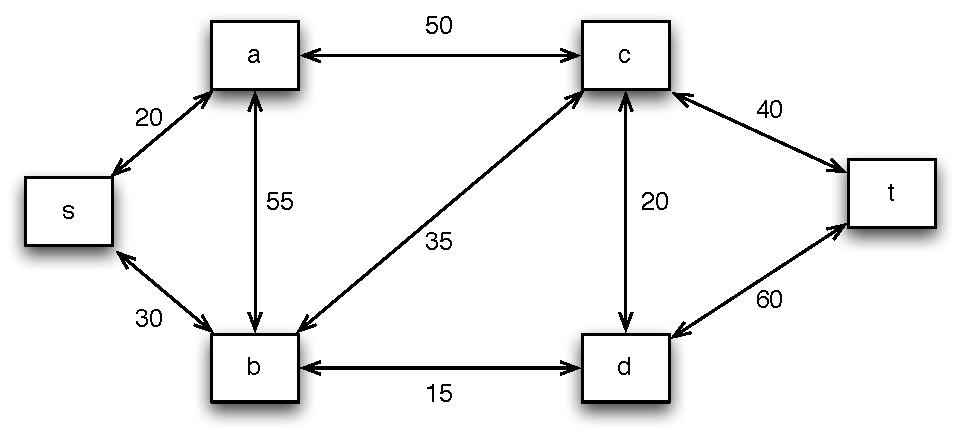
\includegraphics{Dijkstra.pdf}
      }
    \end{figure}

% \textbf{Solution.} 

% \begin{figure}[h]
%       \centering
%       \scalebox{0.7}{
%         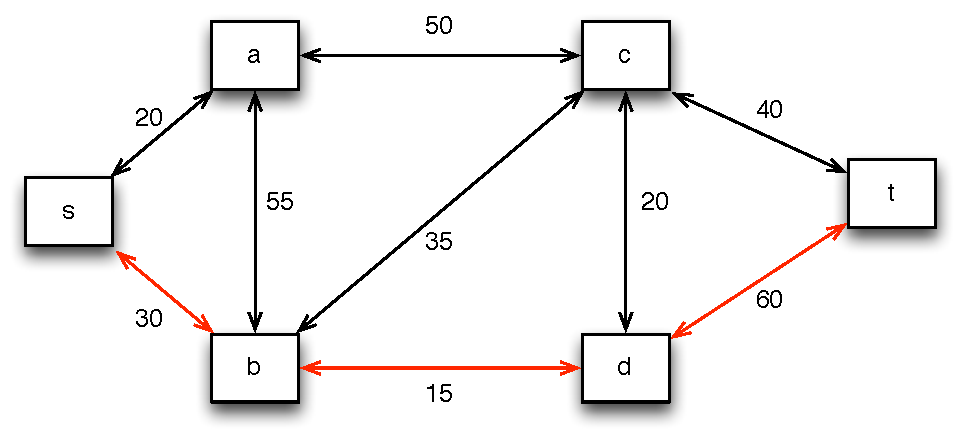
\includegraphics{Dijkstra-s.pdf}
%       }
%     \end{figure}

  \item We have three containers whose sizes are 10 Liters (L), 7 L, and 4 L, respectively. The 7 L and 4 L containers start out full of water, but the 10 L container is initially empty. We are allowed one type of operation: pouring the contents of one container into another, stopping only when the source container is empty or the destination container is full. We want to know if there is a sequence of pourings that leaves exactly 2 L in the 7 or 4 L container.
    \begin{enumerate}[label=(\roman*)]
    \item (2 point) Model this as a graph problem: give a precise definition of the
      graph involved by clearly explaining the vertices and e<dges, and state the specific question about this graph that
      needs to be answered.

% \textbf{Solution.} Let $G = (V,E)$ be our (directed) graph. We will model the set of nodes as triples of numbers $(a_{0}, a_{1}, a_{2})$ where the following relationships hold: Let $S_{0} = 10, S_{1} = 7,S_{3} = 4$ be the sizes of the corresponding containers. $a_{i}$ will correspond to the actual contents of the $i$th container. The following must hold: $0 \leq a_{i} \leq S_{}$ for $i \in \{0,1,2\}$, and at any given node $a_{0}+a_{1}+a_{2} =11$ (the total amount of water we started from). An edge between two nodes $(a_{0}, a_{1}, a_{2})$ and $(b_{0}, b_{1}, b_{2})$ exists if both the following are satisfied:
% \begin{itemize}
% \item the two nodes differ in exactly two coordinates (and the third one is the same in both), and
% \item if $i,j$ are the coordinates they differ in, then either $a_{i} =0$ or $a_{j} =0$ or $a_{i} =S_{i}$ or $a_{j} =S_{j}$. 
% \end{itemize}
%    The question that needs to be answered is whether there exists a path between the nodes $(0, 7, 4)$
% and $(*, 2, *)$ or $(*, *, 2)$ where $*$ stands for any (allowed) value of the corresponding coordinate.
  
\item (1 point) What algorithm should be applied to solve the
      problem?

% \textbf{Solution.} Given the above description, it is easy to see that DFS on that graph should be applied, starting from node $(0, 7, 4)$ with an extra line of code that halts and answers \texttt{yes} if one of the desired nodes is reached and \texttt{no} if all the connected component of the starting node is exhausted an no desired vertex is reached.

    \item (1 point) Find the answer by applying the algorithm.

% \textbf{Solution.} After a few steps of the algorithm (depth 6 on the dfs tree) the node $(2,7,2)$ is reached, so we answer \texttt{yes}.

    \end{enumerate}

  \end{enumerate}    
  
\item (Some simple graph properties: 5 points.) Let $G$ be a graph with $v$ vertices and $e$ edges. Let $M$ be the maximum degree of the vertices of $G$, and let $m$ be the minimum degree of the vertices of $G$. Which of the following propositions must be true? Provide a short proof or counterexample in each case.
	
	\begin{enumerate}
		\item (1 point) $2e/v \le M$
                  % \textbf{Solution.} True. If $v \geq 1$, then $2e/v = \bigl(\sum_{x\in V}\text{deg}(x)\bigr)/v \leq vM/v = M$.

		\item (1 point) $2e/v \ge m$

% \textbf{Solution.} True. If $v \geq 1$, then $2e/v = \bigl(\sum_{x\in V}\text{deg}(x)\bigr)/v \geq vm/v = m$.

\item (1 point) There exists a simple path (includes no cycles) of length at least $m$. 
  
  % \textbf{Solution.} True. Suppose that the longest path in $G$ has length $k < m$. Consider one such path, say $P = x_{1}\dotsb x_{k+1}$ for some labeling $x_{1}, \dotsc, x_{v}$ of the vertices. Consider $x_{k+1}$. Then $x_{k+1}$ cannot be connected to any vertices outside $P$, because this will result in a longer path, contradicting the fact that $P$ is a longest path. Since $\text{deg}(x_{k+1}) \geq m$, it follows that, by the preceding argument, $x_{k+1}$ must be connected to at least $m$ vertices in $P-x_{k+1}$; this is impossible, because $P-x_{k+1} \equiv x_{1} \dotsb x_{k}$ contains $k < m$ vertices. 
  
\item (1 point) $m > 2$ implies that $G$ is connected 
  
  % \textbf{Solution.} False. Consider the graph consisting of two components, each of which is a ``polygon'' (i.e., a cycle) of 5 sides (edges), with an additional center node that is connected by an edge to every node on the polygon. This graph has $m = 3$ but is not connected. 
  
  % Also any graph consisting of two or more components, where each component is a complete graph on $v \geq 4$ vertices is a counterexample. 
  
  % \item (1 point) $M \le v-1$ if $G$ is a simple graph
\item (1 point) In every (simple) graph there is a path from any vertex of odd degree to some other vertex of odd degree.


% \textbf{Solution.} 
% There are many ways to show this; here's one. Let $u$ be a vertex of odd degree in $G$. There must be a component (i.e., a maximal connected subgraph) containing $u$, so take that component. Thus we may assume without loss of generality that $G$ is connected. Recall that the number of vertices of odd degree in any (simple) graph must be even. Since $u$ is of odd degree, there must exist a vertex $v \in G$ whose degree is also odd. There is a path between $u$ and $v$ because they are in the same component, and we are done.


	\end{enumerate}

% \item (Directed acyclic graphs). A directed graph which has no directed cycles is called a directed acyclic graph (DAG). Note that the underlying undirected graph may have cycles.
%   \begin{enumerate}
%   \item Show that in any DAG, there is a vertex whose in-degree equals $0$, i.e., it is not the head for any edge. Such a vertex is called a \emph{source}.  
% \item Show that in any DAG, there is a vertex whose out-degree equals 0, i.e., it is not the tail for any edge. Such a vertex is called a \emph{sink}.

% \item Show that in any DAG, one can order the vertices so as to respect edge directions: i.e., show there exists a one-to-one and onto mapping $f : V (G) \to \{1, \dotsc, n\}$ such that for every directed edge $(u, v)$, $f (u) \leq f(v)$. So every edge points from a lower numbered vertex to a higher numbered vertex. This kind of an ordering is called a \emph{topological sort} of the vertices of a DAG.
% \item We say that a partition of the vertices $V = L_{0} \cup \dotsb \cup L_{k-1}$, where $L_{i} \cap L_{j} = \emptyset$ for all $i \neq j$, is a \emph{stratification} with $k$ levels, if every directed edge $e$ is between vertices in different levels, and the edge points from a lower indexed level to a higher indexed level. Notice that the topological sorting from the previous part is a stratification with $|V |$ levels. Let $G_{0}$ be a DAG and let $L_{0}$ be the set of sources in $G_{0}$. Consider the following graphs. For each $i = 1, 2, \dotsc,$ define $G_{i} = G_{i-1} \setminus L_{i-1}$ and $L_{i}$ is the set of sources in $G_{i}$. Notice that for some natural number $k^{*}$, for every $i \geq k^{*}$, $G_{i}$ is just the empty graph, i.e., empty set of vertices and empty set of edges. Show that $V = L_{0} \cup L_{1} \cup \dotsb L_{k^{*}-1}$ is a stratification.
% \item (\textbf{Bonus}) Show that $k^{*}$ in the previous part is the smallest $k \in \N$ such that there exists a stratification with $k$ levels.  
% \end{enumerate}

\item (BONUS. Some more graph properties: 2 points.) Let $m$ be a positive integer and consider a graph $G^{*}$ with $2m$ vertices: $v_{1}, \dots, v_{2m}$. An edge exists between vertices $v_{i}$ and $v_{j}$ if and only if $(i-j \equiv 1 \mod 2m) \vee (i-j \equiv 2m-1 \mod 2m) \vee (i-j \equiv m \mod 2m)$.
		
		Note that $x \equiv y \mod n$ if and only if $x = kn+y$ for some integer $k$. As examples, $25 \equiv 5 \mod 20$, $29 \equiv -1 \mod 30$ and $29 \equiv 29 \mod 30$.

	\begin{enumerate}
		\item (1 point) For each $j \in \{2, \dots, 2m\}$, what is the distance between $v_{1}$ and $v_{j}$? The {\em distance} between two vertices of a graph is the number of edges on the shortest path that connects the two vertices. (Derive an expression in terms of $i$, $j$ and $m$. You will have to consider a few cases.)

                  % {\bf Solution.} If $j \le \lfloor m/2 \rfloor +1$, the distance is $j-1$. If $\lfloor m/2 \rfloor +1 < j \le m+1$, the distance is $m-j+2$. If $m+1 < j \le \lceil 3m/2 \rceil$, the distance is $j-m$. If $\lceil 3m/2 \rceil < j \le 2m$, the distance is $2m-j+1$.
                  
                  
		\item (1 point) A graph $G$ is $k$-edge-connected if and only if one has to remove $k$ edges to disconnect the graph. Prove that $G^{*}$ is not 4-edge-connected: you can remove three or fewer edges to disconnect the graph.

% {\bf Solution.} Consider $v_{1}$. If $m=1$, remove the single edge to disconnect the graph; otherwise remove the three edges incident on $v_{1}$.

\end{enumerate}


\end{enumerate}



%%%%%%%%%%%%%%%%%%%%%%%%%%%%%%%%%%%%%%%%%%%%%%%%%%%%%%%%%%%%%%%%%%%%%%%%%
%% the bibliography starts here.

%\newpage
%\bibliographystyle{acm}
%\setlength{\baselineskip}{0.8\baselineskip}
%\bibliography{../../Bibliography/CompleteBibliography}

%%%%%%%%%%%%%%%%%%%%%%%%%%%%%%%%%%%%%%%%%%%%%%%%%%%%%%%%%%%%%%%%%%%%%%%%%
%% other closing material

% \appendix
% \input{appendix.tex}

\end{document}
%%% Local Variables:
%%% mode: latex
%%% TeX-master: t
%%% End:
